
\section{Motivation}

% identification of most frequent items
One of the most fundamental subroutines in data analysis is extracting the most frequent items in a data stream. Extracting the most frequent items is used in a variety of machine learning applications, such as feature selection~\cite{thoma2009near}, ranking~\cite{popescu2011text}, semi-supervised learning~\cite{ahmed2015semi}, and natural language processing~\cite{chowdhury2003natural}, but has also been utilized for network monitoring~\cite{li2010mining} and security~\cite{paredes2010automating}. Popular data processing libraries, such as Twitter's Algebird~\footnote{\url{https://github.com/twitter/algebird}}, have also included frequency estimating techniques~\cite{deng2007new}. In addition to its indirect use integrated in some more extensive logic, high-frequency item detection finds practical direct applications, e.g., to answer with efficient approximations  questions such as what are the most searched keywords on the Internet~\cite{rovetta2020covid} as well as how much data is sent between two devices in a network~\cite{mistry2016network}.

% focus on streams
Data volumes keep growing, and so efficiently prioritizing information in a gigantic mass becomes indispensable. Yet, the resources available to filter the data to the most relevant are scarce in the face of the gigantic workload---e.g., in the context of the ever-growing Internet of Things (IoT) where billions of items are to be processed by devices with tightly limited storage, computing and network capabilities.
% 
In this challenging setup, because it is so resource-efficient by design, the stream processing paradigm, where every item is seen only once, has established itself as one of the most prominent forms of data processing. Determining the most important items in that context means tracking in real time the most important items when fed with infinite streams, i.e., only a finite amount of state can be kept even though the input is assumed to be of infinite size.
% 
In use cases like the detection of denial of service (DoS) attacks or identifying the most frequently purchased products in a stream, the importance of an item is typically its count, leading to the \emph{heavy hitter} detection problem.

% learned databases
An approach receiving particular attention lately to monitor the heavy hitters in a data stream efficiently consists in learned sketch models~\cite{hsu2019learning,kristo2020case,patil2021latest} where the data is represented in a latent form, i.e., as a learned model---typically a neural network--- as opposed to the traditional explicit form of sketches---e.g., Count-Min Sketch~\cite{cormode2005improved}, or Space Saving~\cite{mitzenmacher2012hierarchical}. The model is trained to learn the data patterns, i.e., the usual ingestion is replaced by some training, and the model is able to return data when requested, i.e., queries are traded for inferences; hence, an entire database is emulated by a model.

% models for streams
With the major significance of the streaming scenario and the high interest for models serving as learned databases has come a stringent need for models at the intersection, namely serving as databases taking in streams. In a streaming scenario, the pattern, or distribution (concept) to be learned by the tracking model changes (drifts) significantly over time: there is a concept drift~\cite{Widmer1996,yu2021automatic}, and particularly so compared to, e.g., a mostly static database.
The domains in which the data to be processed changes over time are very diverse. Invariably, though,
the data patterns are that the data changes very fast, e.g., in the Internet field, as flash crowds in Internet traffic as a whole~\cite{ari2003managing}.
This also holds in the myriad of fields with similar characteristics, e.g., marketing~\cite{kotler2005role} or recommendations on social media~\cite{}.
%
As indirect applications of most frequent element tracking, some well-known applications include frequent items, heavy changers, persistent items or super-spreaders~\cite{li2020wavingsketch}.
%
Yet, frequent estimation is too coarse on its own to satisfy meaningfully the breadth of use cases practitioners are confronted with. A key problem downstream of frequency estimation is to distinguish a genuine flash crowd~\cite{ari2003managing,oikonomou2009modeling}, which needs to be served, from a (Distributed) Denial of Service attack, which needs to be blocked. A refined modeling of data patterns is then necessary, typically looking at human-characteristic temporal patterns in the connection, to try to block malevolent flows~\cite{tandon2021defending} or to give users appropriate feedback when delays occur~\cite{tada2021mitigation}. And yet, even many more aspects would need to be taken into account to correctly represent the behavior of the target population~\cite{aljohani2021conducting} than is currently integrated in existing monitoring systems.
% 
In that context, while constant progress on actual estimations to make them more accurate for a lower amount of resources~\cite{huang2018sketchlearn,li2020wavingsketch} is beneficial, it is more the efficiency of larger pipelines that these estimations are integrated in that should be optimized. Unsurprisingly, some work has tried to optimize tracking performance for more high-level queries~\cite{zhao2021cluster,zhang2021cocosketch} and attempting to capture a holistic situational view leading up to events~\cite{husak2021system}. Yet, there is a need for a representation with much higher expressivity to really model a non-trivial fraction of the information and processes at play in organizations nowadays~\cite{turunen2021minimum}, generally in a vast array of microservices~\cite{debroy2019overcoming} and a highly heterogeneous set of processes as seen by different actors~\cite{sousa2019managing}.

% why latent driven by explicit is necessary
Hence, beyond frequency tracking, a more extensive modeling of the data is necessary and there the frequency is only one drive out of many in the model. There is a need for models where driven by simple metrics but with a representation that allows full expressivity. Typically, queries are generated interactively~\cite{kraska2021northstar}, e.g., to look for an interesting pattern (such as an anomaly) and approaches trying to store the data to optimize for queries~\cite{zhao2021cluster,zhang2021cocosketch} do not offer this flexibility in their expressivity because only a fraction of the information is maintained. A broader and more holistic representation of the entirety of the data is necessary and there the clear and easily understandable shallow metric of importance that the frequency is should be the drive, i.e., the weight, from which the importance of the data is derived (backwards attribution), and not the target, i.e., what is represented. There, a latent representation---in the continuity of the booming field of database learning~\cite{hilprecht2019deepdb,hasan2020deep}---is appropriate but, most importantly, this latent representation needs to be driven by an importance metric.
% in continuity with the discussion in Nebi's work, going further; latent vs. explicit


% concept drift in latent representation
When it comes to latent representation, yet, changes on the data become per nature hard to carry over, unlike regarding porting changes in the data to explicit representation such as a list: local changes in the data can have an arbitrary impact in the latent space. The most important case of data changing is when the dataset to represent is dynamic: the distribution of the dataset to store---the concept--- varies over time---drifts---: there is a concept drift.
%
Existing work attempting to represent the data driven by the simple importance metric that is the frequency~\cite{hsu2019learning} fails to account for the concept drift and is content with building a single model supposed to cover the distribution forever.
%
Yet, these shifts can be considerable and changes in the underlying distribution would have a detrimental impact on the model's performance: the underlying distribution drifts further and further away from the learned model.


% general approaches in literature
\subsection{General Strategies which can be applied for handling Concept Drift}

% current methods to concept drift and their cons
To prevent the model from becoming progressively obsolete, the usual approach is to update it on a regular basis.
% 
As a result, it is necessary to i) capture concept drift and ii) update the model in a way that is tailored to the concept drift observed---for example, discarding the most obsolete parts of earlier learning and attempting to learn what appears to be the most significant next.
% 
The state of the art has touched upon identifying the most critical elements to forget and learn by employing a time-aware transformer architecture over sequences~\cite{zhang2020time,ren2021rapt,sawhney2020time}.
% 
However, these methods do not offer a high degree of generality in capturing concept drift, nor do they provide a differentiated and understandable degree of control in the forgetting and learning driven by an explicit importance metric.


% shortcomings of previous approaches
\section{Problem Statement}

Explicit frequency-driven sketches store only a narrow fraction of the data according to a prioritization scheme defined a priori per hand, and that precludes the migration to any subset of the data prioritized in even a slightly different manner.

Deep learning models are the opposite of this overly discrete representation in that they are designed for a very efficient representation of latent patterns. Hence, deep learning models are able to represent efficiently the data in the full extent of its complexity. Yet, as a natural consequence of their design optimized for latent representation per construction they catch on a broad array of patterns to support efficient prioritisation w.r.t. any prioritisation metric, e.g., lacking explicit error boundaries.

The problem of the lack of prioritization in the representation is particularly acute when there are changes involved which is by far the default situation as both data and queries change quickly at all time. There, an explicit representation handles the evolution optimally but the concept drift then damages the model in a latent representation and without any principled and efficient notion of prioritization, the model is unable to maintain a high quality in areas close to the areas of importance in the latent space, a problem only solved by very generous learning to correct the model, at high cost.

Hence, there is a need for a model bringing together explicit representation and latent representation in an optimized combination where (i) the explicit representation drives the importance estimation of the combination and the latent representation generally follows the lead of the explicit representation for the importance estimation (the explicit representation is also closer to the interaction with the environment, hence more readily and precisely impacted by the environment) but (ii) but in the same time the latent representation serves as a much needed complement to store more broadly around what the explicit representation considers important.
This combination should optimize itself in tandem and continuously updates itself as changes come in.

Hence, we propose to address the following problem:
% 
\begin{quote}
    \itshape{How to dynamically track top items in an optimized blend of latent and explicit representation?}
\end{quote}



\section{Solution}

We want to keep only the top most important items at all times. At the same time, guarantees should be provided in our vertical. We backtrack from top to the mass, which can be interpreted as from discrete to continuous. The tracking and data are both dynamic.

To deliver the feedback explicit/latent, we offer a vertical combination: a latent representation of the items in the form of a neural network learning the distribution as its neural state, and a sorted list of top items to represent the items explicitly. The explicit part backpropagates feedback from the top items to the latent representation. The latent representation is queried to complete the explicit part in proportion of the error guarantees that the explicit part produces.

Note that this sort of back-and-forth feedback between an explicit and a latent part with mutual (or even one-sided) influence is very powerful: it allows small and understandable actions onto restricted and specific parts of the explicit representation (by a human user or by a machine) to have their impact propagate in the vicinity of these specific parts in the explicit representation, but this vicinity is taken in the combination of the explicit and latent representation and thus of very high semantic coherence. Hence, understandable actions in the simple space (explicit representation) that is the explicit representation can have a very intricate impact but with the intricacy driven by an understandable logic (explicit representation). (In a visual context, this latent logic could also be a logic abstracted away and not shown~\cite{kraska2021northstar} rather than a neural network.)

We use state-of-the-art mechanisms for updating both the latent representation and the explicit representation. For the latent representation, we use a time-extended representation of both input and state but also relearning when necessary. For the explicit representation, we make use of data structure maintaining lists of items according to a fixed score with statistical guarantees, sketches.

% system design
We propose a solution which addresses the requirements in a unified and flexible manner:
(i) we deliver a combined representation where the top tracked by the explicit representation is used as a reference to evaluate and propagate back into the latent representation (Section~\ref{sec:cooperation_latent_explicit_representation}),
(ii) we deliver a representation able to efficiently update itself (Section~\ref{sec:extensive_temporal_encoding}).

\begin{itemize}
  \item optimized hybridization model-based and neural network
  \item optimized tracking top vs. mass
  \item augmented concept drift tracking
  \begin{itemize}
    \item t-LSTM 
    \item incremental learning
  \end{itemize}
\end{itemize}


\subsection{Cooperation Latent/Explicit Representation}
\label{sec:cooperation_latent_explicit_representation}

\subsubsection{Re-labeling and train}

We build upon the state of the art in database modeling in the form of Learned Sketch~\cite{hsu2019learning}.

The output of Learned Sketch diagram are estimated counts, which is an elementary example of an importance metric. Using internal work, we will expand to importance metrics combining frequency and an estimate of the user's interest by a Markov chain modeling the user's sequential behavior.

To improve the performance of training, we want to use neural networks combined with sketches to train the neural network, i.e., instead of feeding the ground-truth counts as labels to the network, as they currently do, we feed the counts (the output of sketches) that we get from the whole system.


% next steps: extend stub up to top
\subsubsection{Extend stub up to top}

\paragraph{Simple Top Backpropagation: Hybrid Semi-supervised Loss}

% 
After building the neural network, how to train the model is another important theme. In general, the learning techniques are divided into two types, namely i) supervised training and ii) unsupervised training. The fact that there is or there is no supervision depends on the inputs.

From the perspective of inputs, by supervised training, a predefined set of labels will be fed into the model so that the model produces the output from the previous experience, while by unsupervised training the model learns all kind of pattern from the data without using labels. 

We use the sparse cross entropy. We change the frequency estimates of deciding the probability of belonging to classes. Here, the classes are simple: in top vs. in bottom. For different values of the number of items in the top, k, we get different ground truth top and ground truth bottom. And for the same frequency estimates, for different values of the number of items in the top k, we get different estimation of top and estimation of bottom. 

\paragraph{Top-F1 metric on top of the model}

We want to create a new metric called top-F1 that would take in ground truth and estimated frequencies and, being parametrized by a control parameter k, first generates the probability labels for estimation and ground truth, and then calls an F1 computational method.

We add a layer on top of the regression (to frequency estimates) to return the top k (form of pooling) and then another layer on top to compute the top F1. Then, we would be able to use as loss weighted sum of top F1 and MSE, possibly with automated meta optimization. The system is then rewarded for improving on the items that matter most.



\subsection{Extensive Temporal Encoding}
\label{sec:extensive_temporal_encoding}

\subsubsection{Positional Encoding of relevant Subsets in an organic Order}

% RNN, LSTM or transformers
To encode the positional information, existing work~\cite{zhang2020time} only considers the time difference between subsequent items. This is insufficient, e.g., for the case that there are more irrelevant items in-between: item at t1, item at t2, item at t3; with item at t1 and item t3 related. Further, the chronological order might well not be the best inductive path, e.g., symptom at t3, symptom at t1 and symptom at t4 could be a sequence where each next step is more logically derived from the last than with the same items simply in the chronological order---think questions that a physician would ask: they absorb the information in the order that the attention conditioned by the information obtained would impose, not in the chronological order. Hence, the only solution for high expressivity in sequence capture appears to be to identify relations over subsets fed as a sequence but in an order dictated by an organic stateful attention. Each time, we would encode the organically generated sequence by applying recurrent encoding (RNN, LSTM or transformers, depending on availability) to capture the positional information efficiently.

\subsubsection{Combined Timestamp and Value Encoding} \label{sec:timestamp_encoding}

Since time information of each observation (submissions in the context of CAIDA trace) could play some role in drift analysis, a sensible solution is to encode the timestamps as part of the observation itself, i.e., as one additional feature. Then, the model is made \emph{explicitly} aware of the time associated with each update.


% Adaptive Re-Learning
\subsection{Adaptive Incremental Learning}
\label{sec:adaptive}

Our system should adapt to new data in real time. At training time, from the nature itself of incremental learning, the system would gradually learn from one batch to the next, with each time the model adapting more to fit the latest batch and incidentally potentially less to fit earlier batches. This also happens if the batches are episodes, i.e., sequences of observations.

This better fit to the latest batches fed in is usually something rather undesirable because it corresponds to overfitting on the latest batches, which would result in lower performance on the test batches. The usual means to avoid that effect is to order the batches at random, or, better in terms of sample efficiency, to select as much as possible batches that challenge the system at any point in time (see the line of work of Generative Adversarial Networks).

Yet, the overfitting on the latest batches can be a phenomenon to capitalize upon: the model could be re-trained to a variety of degree (each to be amortized appropriately over time), with more or less heavy supervision, over later batches.

Overfitting on latest batches would happen naturally if the dataset fed is ordered chronologically. To weaken or reinforce this overfitting, as needed, we would do heavy/light learning on recent batches vs. redo heavy/light learning on older batches.




\section{Early results}
\label{sec:results}

We implemented a prototype with partial functionalities on a latent/explicit ecosystem and concept drift tracking, using incremental learning, and we evaluated its capacity to deliver a better performance than vanilla versions.

\subsection{Prototype}

We use a flexible input encoding logic adapted to the input, e.g., a RNN. Afterwards, we use three-layer fully-connected networks to encode the feature vector.

We train the whole neural network to predict the log of the item counts.


\subsection{Latent/Explicit Ecosystem: Top backpropagation}
%from learned sketch and added my portion

To give the system an incentive to get better on the items that really matter, on top of the regression (old Learned Oracle neural network), we added sorting \& classification  (parametrized only by k, so no weights here) into the model to compute the top F1. Then, we would be able to use as loss weighted sum of top F1 and MSE, possibly with automated meta optimization. 


\subsection{Concept Drift: Adaptive Incremental Learning}

We train our system with new data continuously. To do this efficiently, we first specify a dynamic window size based on the amount of new data being generated. At the end of each window, we train our system~\cite{misra1982finding,fan2000summary}. The embedding of sequences containing new items is postponed until the window boundary where we can afford to use more resources
%  [from Timo]

The aim of incremental learning is for the learning model to adapt to new data without forgetting its existing knowledge. It can begin with a very small set of samples, and grow its knowledge as more data is absorbed. The ability to evolve based on more data also results in higher accuracy.


\subsection{Implementation}

\paragraph{Upgrading existing Code Base to TensorFlow 2}

We use as a starting code basis the code from Learned Sketch~\cite{hsu2019learning}.

% https://towardsdatascience.com/everything-you-need-to-know-about-tensorflow-2-0-b0856960c074
TensorFlow~\cite{tensorflow2015-whitepaper} is a general-purpose high-performance computing library open-sourced by Google in 2015. Since the beginning, its main focus was to provide high-performance APIs for building Neural Networks (NNs). However, with the advance of time and interest by the Machine Learning (ML) community, the library has grown into a full ML ecosystem.

Compared to TensorFlow 1.0, TensorFlow 2.0 focuses on simplicity and ease of use, with updates like eager execution, intuitive higher-level APIs, and flexible model building on any platform. There are multiple changes in TensorFlow 2.0 to make TensorFlow users more productive.

% from TensorFlow 1.0 to TensorFlow 2.0
\paragraph{Full Use of Modern TensorFlow Utilities}
In order to be able to transfer feedback conveniently, we upgraded the entirety of the Learned Sketch code from TensorFlow 1.0 to TensorFlow 2.0 and added some other improvements: 1)refactor the code into smaller functions 2)use Keras layers and models to manage variables 3)combine tf.data.Datasets and tf.function 4)take advantage of AutoGraph with Python control flow 5)tf.metrics aggregates data and tf.summary logs them 
% https://medium.com/featurepreneur/tensorflow-1-0-vs-tensorflow-2-0-240fc6efb14f


\subsubsection{Data Preprocessing}

\paragraph{Data}
The traffic data is collected at a backbone link of a Tier1 ISP between Chicago and Seattle in 2016 (CAIDA). Each recording session is around one hour. Within each minute, there are around 30 million packets and 1 million unique flows.

\paragraph{Preprocessing}
We preprocessed the features and counts of each unique internet flow in each minute. To rearrange raw data in chronological-window order, we designed the following automated preprocessing parser:

\begin{enumerate}
    \item extracts data from file: 8 byte for timestamp, 4 bytes for source IP, 4 bytes for destination IP
    
    \item extracts data from window out of the dataset 
    
    \item separate data into windows of predefined length
    
    \item Writes the 1000 most frequent flows with their total occurrence in the destination file.
\end{enumerate}

\paragraph{Encoding}

The model takes as input the IP addresses and reshape them to fit in the Keras network. We use two RNNs which consist of LSTM cells to encode the source and destination IP addresses separately. The RNN takes one bit of the IP address at each step, starting from the most significant bit. We use the final states of the RNN as the feature vector for an IP address. The reason to use RNN is that the patterns in the bits are hierarchical, i.e., the more significant bits govern larger regions in the IP space.

The items are flows and when packets are seen as belong to a flow they update the attributes of that flow. I.e., the items gets updated.


\subsubsection{Metrics}
% derive metrics from problematic, i.e., what we are interested in
We want to evaluate the ability of the systems to represent correctly the most important items.
Hence, we look at how often items are labeled as in the top vs. bottom category for various sizes of the top (k): we consider the area under the curve (AUC) for the problem of labeling as in the top based on estimates from our representation.


\subsubsection{Evaluation of the ability to adapt with Concept Drift}

% ## Concept Drift Evaluation – Exp. 1
\paragraph{Concept Drift Evaluation 1: Evaluating the Impact of Incremental Learning Standalone}

% Please always discuss each experiment by following this process:
% 1. Say we want to investigate sth. and why it will bring us useful insights.
% 2. Say how we investigate that thing, i.e., experimental setup.
% 3. Say our results are presented in Material XYZ (plot/table)
% 4. describe the results. Just tell us what are the most striking patterns
% 5. discuss the results. Try to explain what we saw


% 1. Say we want to investigate sth. and why it will bring us useful insights.
We want to study the impact of incremental learning, i.e., training on recent data, on the convergence behavior, i.e., how fast the model converges and with what performance while training but, more importantly, when testing subsequently.

% 2. Say how we investigate that thing, i.e., experimental setup.
We design our experiment as follows. We compare a model that learns from an earlier window with a model that learns from a recent window, and we test each time on a window later in the sequence.
In the no incremental learning setup, we train the model over window 1, then test on window 20; in the full incremental learning setup, we train on window 19, then test again on window 20.

% 3. Say our results are presented in Material XYZ (plot/table)
We present our results in Figure~\ref{fig:comparison_concept_drift}.
% 
\begin{figure}[htbp!]
     \centering
     \begin{subfigure}[b]{0.5\textwidth}
         \centering
         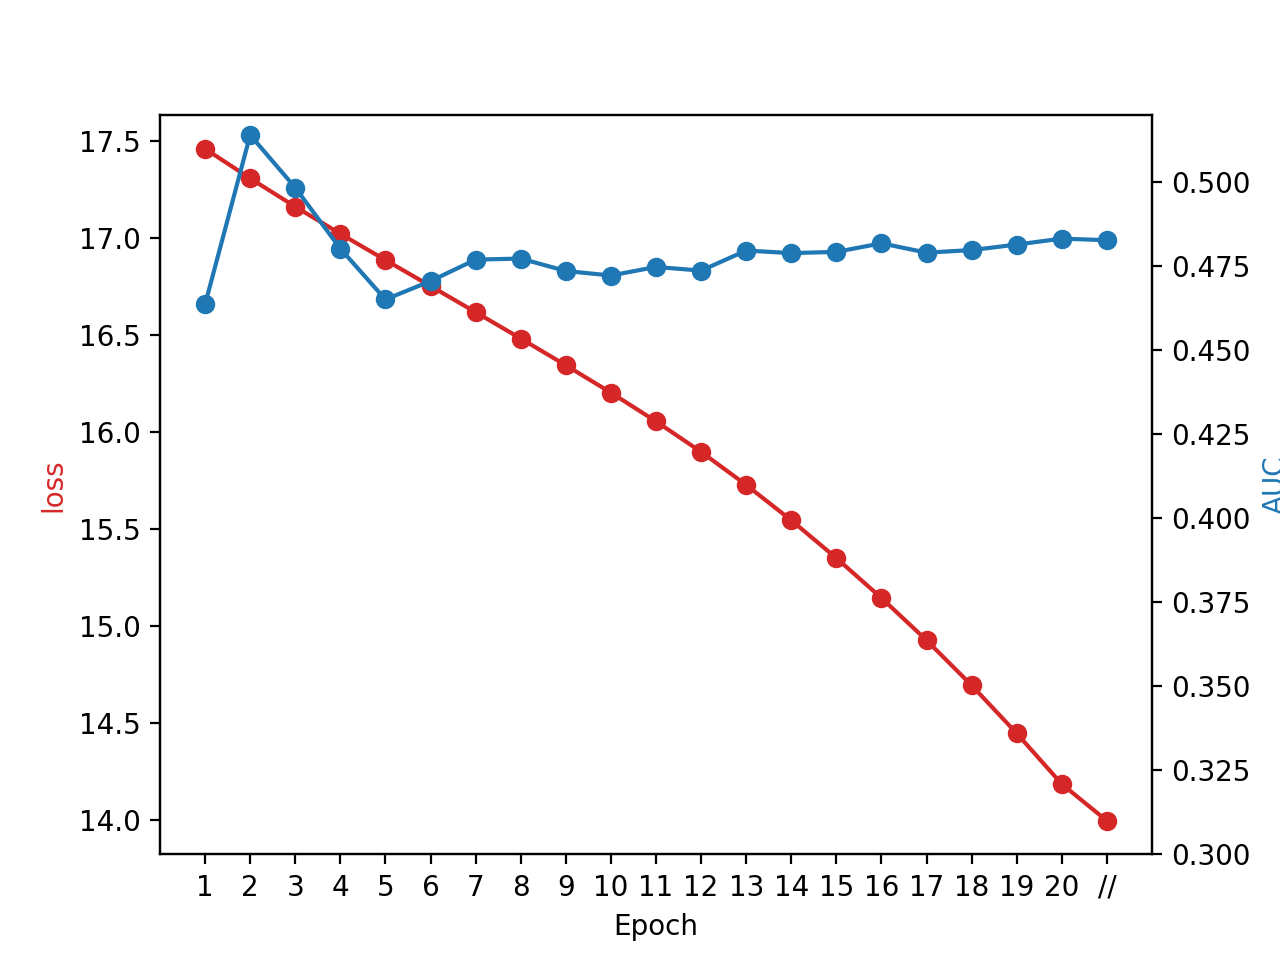
\includegraphics[width=\textwidth]{images/plots/train1_test20.png}
         \caption{Train on window 1, test on window 20}
         \label{fig:train_1_test_20}
     \end{subfigure}
     \hfill
     \begin{subfigure}[b]{0.5\textwidth}
         \centering
         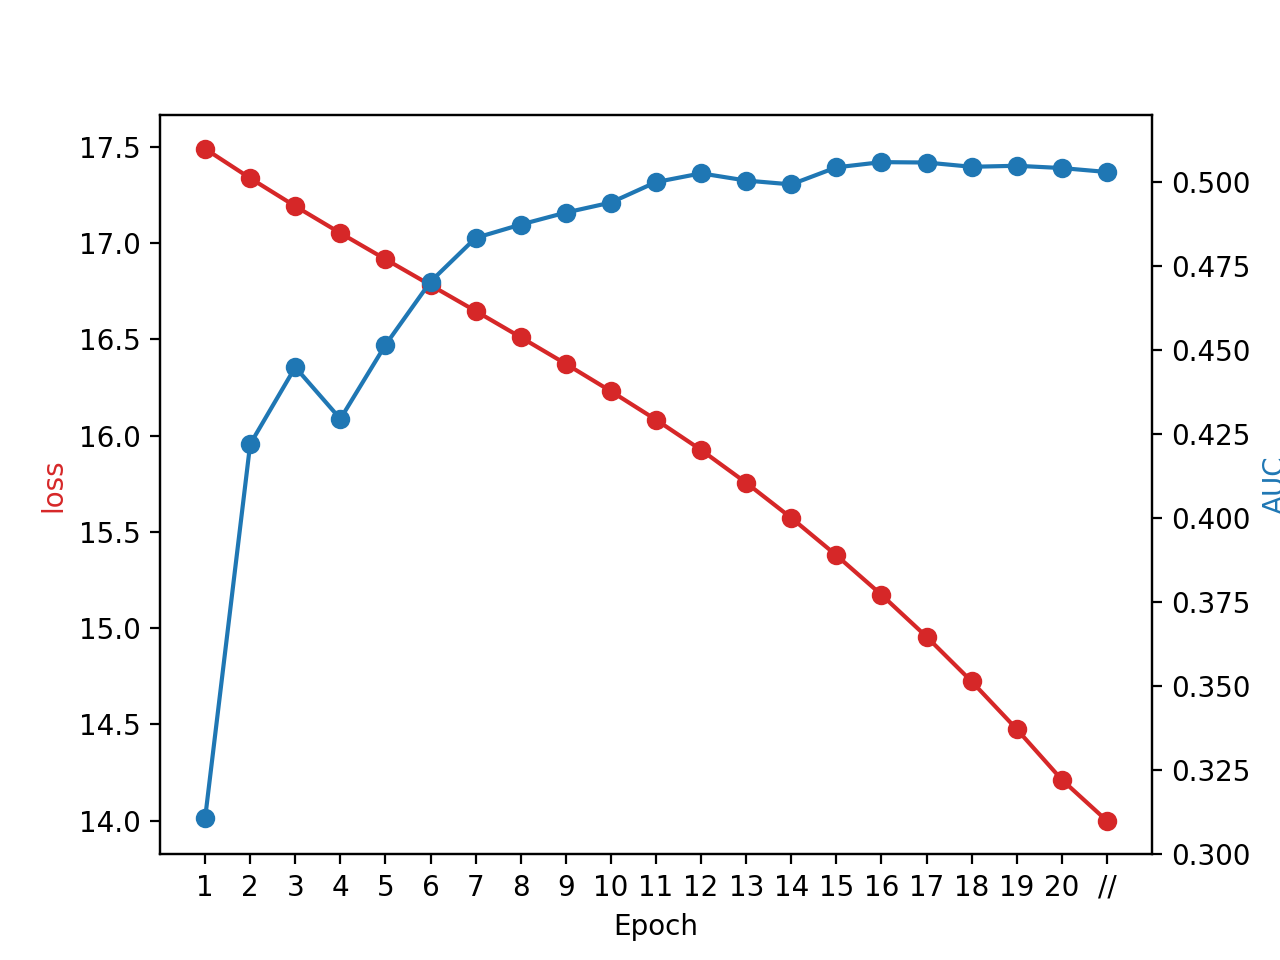
\includegraphics[width=\textwidth]{images/plots/train19_test20.png}
         \caption{Train on window 19, test on window 20}
         \label{fig:train_19_test_20}
     \end{subfigure}
    \caption{'Illustration of the impact of more or less incremental learning on the convergence behavior'.  Before  the axis break ('//') is presented the performance at train time. After the axis break the performance at test time.
    (left) No incremental learning: Training the model on window 1, then testing on window 20.
    (right) Full incremental Learning: Training the model on window 1, then testing on window 20.}
    \label{fig:comparison_concept_drift}
\end{figure}

% 4. describe the results. Just tell us what are the most striking patterns
As epochs pass, we can see AUC score increase faster and converges at a higher value in full incremental learning setup (i.e., training on window 19 which is more recent to the test window). While that's a less significant aspect about the performance in general, the AUC score at testing time in the full incremental learning setup is also higher than in the no incremental learning setup.


% 5. discuss the results. Try to explain what we saw
The system with incremental learning outperforms the system without incremental learning regarding AUC score, which verifies the impact of incremental learning on addressing concept drift.


% ## Concept Drift Evaluation – Exp. 2
\paragraph{Concept Drift Evaluation 2: Evaluating the Impact of the Horizon after convergence}

To analyze the impact of keeping more or less outdated information, we let our model train on older windows and be tested on newer windows, and we let the number of windows in-between (the horizon) vary.

(Note that this corresponds to giving more or less episodic memory to the model).

In the interest of simplicity, we keep the training on older windows constant and restricted to learning only on a batch of one window. We test on window sets further and further ahead of the old window; for now only one window each time.
% 
Hence, in our simplified experimental setup, we train on Window 1 and test in turn on Window 2, on Window 3, etc.

We present the performance by plotting the AUC score against the index of the window tested.
Our results are illustrated in Figure~\ref{fig:AUC_onFurther_windows}.

\begin{figure}[htbp!]
	\centering
	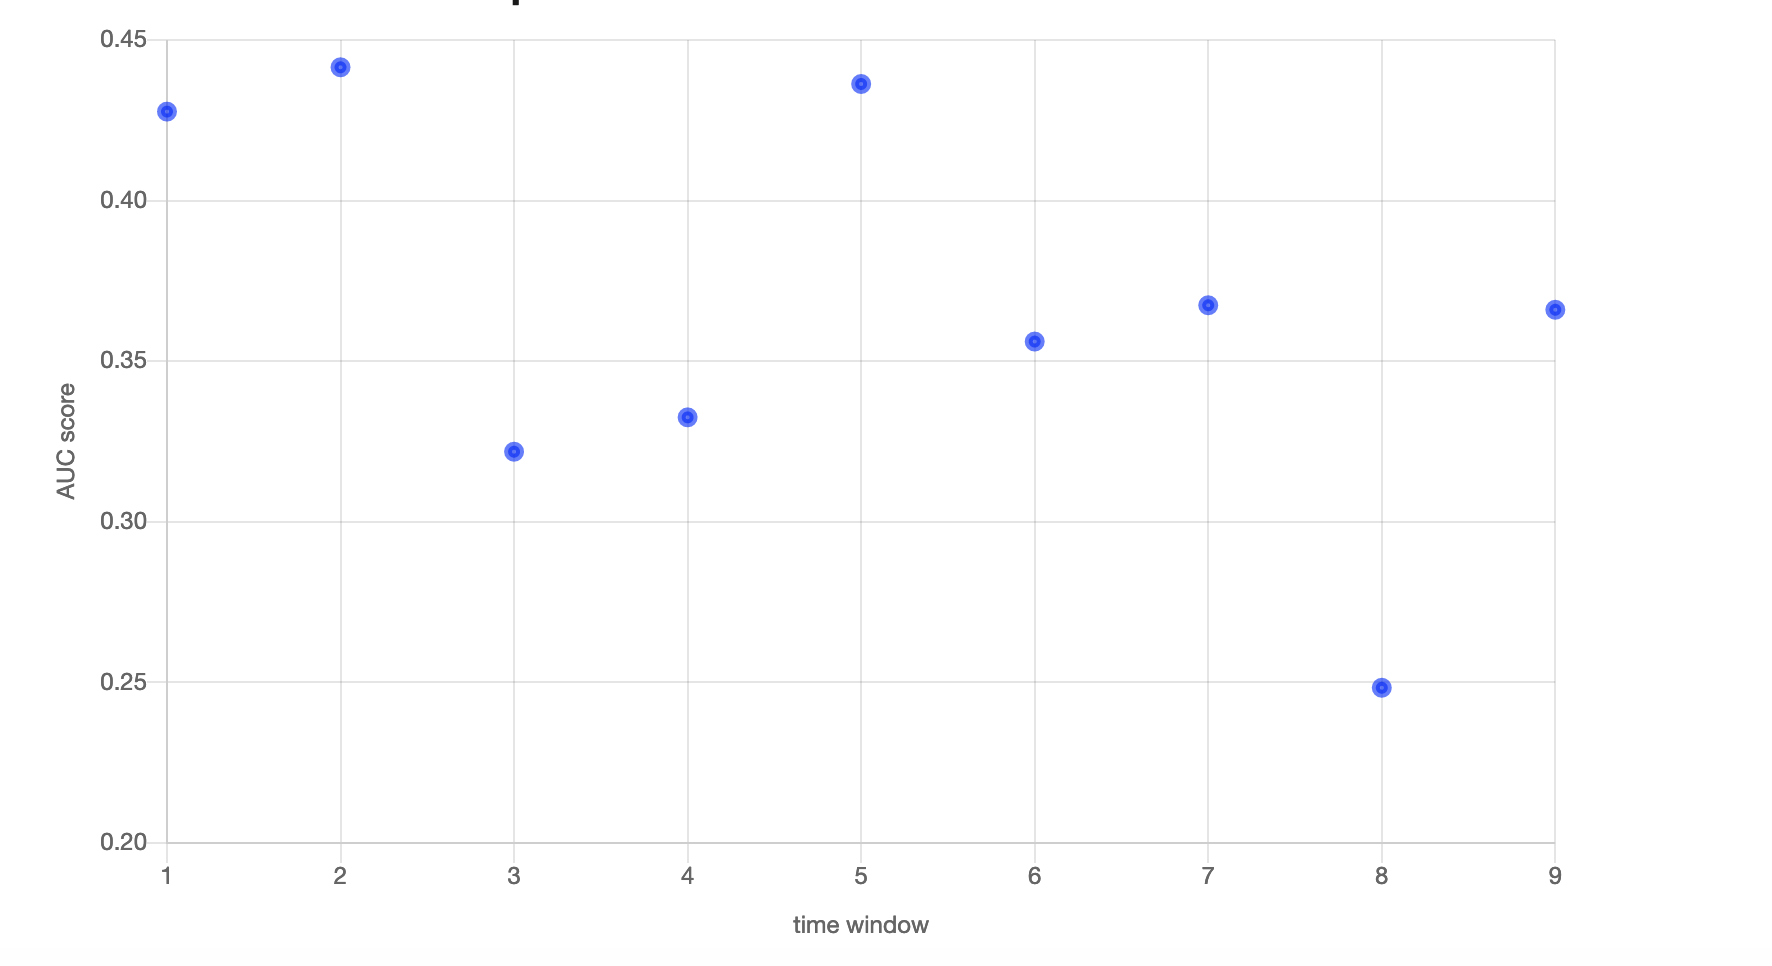
\includegraphics[width=0.6\linewidth]{images/plots/concept_drift_capture.png}
	\caption{Illustration of the impact of concept drift on the representation quality: AUC for testing windows further and further ahead from the train window.}
	\label{fig:AUC_onFurther_windows}
\end{figure}

The AUC appears to decrease as we are testing on later and later windows.

This confirms the concept drift: The dependency of the output on time changes over time, the model will not be able to capture this change, thus the trained model performs worse when the time window slides by. So, we succeed to capture concept drift. 


\subsection{Evaluation of the explicit/latent Ecosystem}

\subsubsection{Upgrading TensorFlow Framework}

% https://towardsdatascience.com/everything-you-need-to-know-about-tensorflow-2-0-b0856960c074
TensorFlow~\cite{tensorflow2015-whitepaper} is a general-purpose high-performance computing library open-sourced by Google in 2015. Since the beginning, its main focus was to provide high-performance APIs for building Neural Networks (NNs). However, with the advance of time and interest by the Machine Learning (ML) community, the library has grown into a full ML ecosystem.

Compared to TensorFlow 1.0, TensorFlow 2.0 focuses on simplicity and ease of use, with updates like eager execution, intuitive higher-level APIs, and flexible model building on any platform. There are multiple changes in TensorFlow 2.0 to make TensorFlow users more productive.

% from TensorFlow 1.0 to TensorFlow 2.0
In order to be able to transfer feedback conveniently, we upgraded the entirety of the Learned Sketch code from TensorFlow 1.0 to TensorFlow 2.0 and added some other improvements: 1)refactor the code into smaller functions 2)use Keras layers and models to manage variables 3)combine tf.data.Datasets and tf.function 4)take advantage of AutoGraph with Python control flow 5)tf.metrics aggregates data and tf.summary logs them 
% https://medium.com/featurepreneur/tensorflow-1-0-vs-tensorflow-2-0-240fc6efb14f

% new section
\subsubsection{Pooling the top-k}

To give the system an incentive to get better on the items that really matter, on top of the regression (old Learned Oracle neural network), we added sorting \& classification  (parametrized only by k, so no weights here) into the model to compute the top F1. Then, we would be able to use as loss weighted sum of top F1 and MSE, possibly with automated meta optimization. 


The test loss decreases from 15.89 to 0.24. But the top-K F1 score is quite low, which indicates that the performance of sorting and classification is insufficient. It could be because the weights of MSE and top F1 are still not optimized. We will do the improvement in the later optimization.


\section{Next Steps}

In general, we would like to extend our experimental setup to include baselines from the state of the art.

\subsection{Next Step in Concept Drift: Adaptive Re-Learning}

We will adapt to recency-prioritized learning in our model by picking most recent batches with a higher likelihood, using an appropriate batch dispatching strategy.

In the process, we will extend our evaluation to a fully-fledged benchmarking effort: by extending our evaluation, we have more information to optimize with.


\subsection{Next Step in Top Pooling: Importance-optimized learning with Guarantees}

After customizing loss with a weighted sum of MSE and top k F1 score, the model performance can still be improved by applying an importance-optimized form of learning --use output of Sketches instead of gt counts. We belong to the tradition of \emph{Generative Adversarial Networks}~\cite{goodfellow2014generative} trying to zero out on the most relevant examples to learn on, but we go further by modeling importance in an explainable manner. We try to do about the same but with a prioritization not fully inferred but partially inferred in an optimized manner: with a selection inferred by the system itself to the best of its capacity, but values efficiently approximated with guarantees.

Since we were very interested in the ability of latent to represent the data in a more diffused manner, we also plan on experimenting with queries where the importance metric is not directly something as simple and explicit as frequencies but a combination of frequencies and a Markov chain (as in IDEBench~\cite{eichmann2020idebench}, for example).

% = queries a bit further from important, more or less far away
% following more or less Markov chains of users as in our paper we should resubmit, [Sets_Paper_meta_learning](https://www.overleaf.com/9176551421pgnmzvqjkrvr), _Fig. 8_; `tex_sections`/`evaluation.tex`/`fig:plot_w2_vs_mae`
% 


% D.
% there is work in pooling that we should have a look at and use
% like [Hierarchical graph pooling with structure learning](https://arxiv.org/abs/1911.05954)~\cite{zhang2019hierarchical}
% at least to discuss and make sure we borrow everything we can from them and add value on top of them,i.e., 
% bring in stuff they don't.